%%%%%%%%%%%%%%%%%%%%%%%%%%%%%%%%%%%%%%%%%%%%%%
%                insertmeeting
% 1) Title (something creative & funny?)
% 2) Date (MM/DD/YYYY)
% 3) Location (ex. Hagerty High School)
% 4) People/Committees Present 
% 5) Picture 
% 6) Start Time & Stop Time (ex. 12:30AM to 4:30PM)
%%%%%%%%%%%%%%%%%%%%%%%%%%%%%%%%%%%%%%%%%%%%%%
\insertmeeting 
	{Update Utopia} 
	{11/09/21}
	{Hagerty High School}
	{Annika, Anouska, Clayton, Falon, Jensen, Nathan, Ritam, Rose, Samantha}
	{Images/RobotPics/robot.jpg}
	{2:30 - 4:30}
	
\hhscommittee{Multimedia}
\noindent\hfil\rule{\textwidth}{.4pt}\hfil
\subsubsection*{Goals}
\begin{itemize}
    \item Our meeting goals were to make updates to our team information, for example our team Spellbook summarizing our Outreach events and design buttons for the upcoming competition. 

\end{itemize} 

\noindent\hfil\rule{\textwidth}{.4pt}\hfil

\subsubsection*{Accomplishments}
In order to make our table more interesting and informative for scouts from other teams and other spectators, our main task was to update our Outreach Spellbook. We decided to update the photos on some of our past events and change the wording on some of the event descriptions. This is helpful because it keeps our community up to date with the Outreach events that we have hosted, or have been a part of. 


\hhscommittee{Hardware}
\noindent\hfil\rule{\textwidth}{.4pt}\hfil
\subsubsection*{Goals}
\begin{itemize}
    \item fix broken back plate
	\item Add camera mount to back plate
 

\end{itemize} 

\noindent\hfil\rule{\textwidth}{.4pt}\hfil

\subsubsection*{Accomplishments}

As we predicted, a problem with the hardware came up only one day after giving the software team time to create the autonomous program. The poor wood that we made the back plate out of had cracked after extra stress from testing the arm (Figure \ref{fig:pic1}). Although this is a setback, it is a very minor one, and it provides us with an opportunity to create a better way to mount the webcam to the robot. Before, we had the webcam double sided taped to the back plate, allowing it to see the team shipping element during autonomous. Although this had worked well enough, it looked a bit precarious as the camera just hung off the back of the robot , leaving it pretty vulnerable to crashes and collisions (Figure \ref{fig:pic2}). To fix both of these issues at once, we reCADed the backplate adding a hole for the camera to see through so that it can sit on the inside of the robot, protected from collisions. We also extended the plate at the bottom to prevent elements from getting stuck under the robot, as we have observed during driver practice. Finally, we took out some of the pocketing, giving the part more support (Figure \ref{fig:pic3}) and laser cut it out of higher quality wood.
Once the part was laser cutting, we attached the camera onto the plate and screwed the plate onto the robot. Using some zip ties and some holes we drilled in the plate, we attached a strip of surgical tubing onto the part of the plate where the arm hits most to soften the impact a bit (Figure \ref{fig:pic4}).

\begin{figure}[ht]
\centering
\begin{minipage}[b]{.48\textwidth}
  \centering
  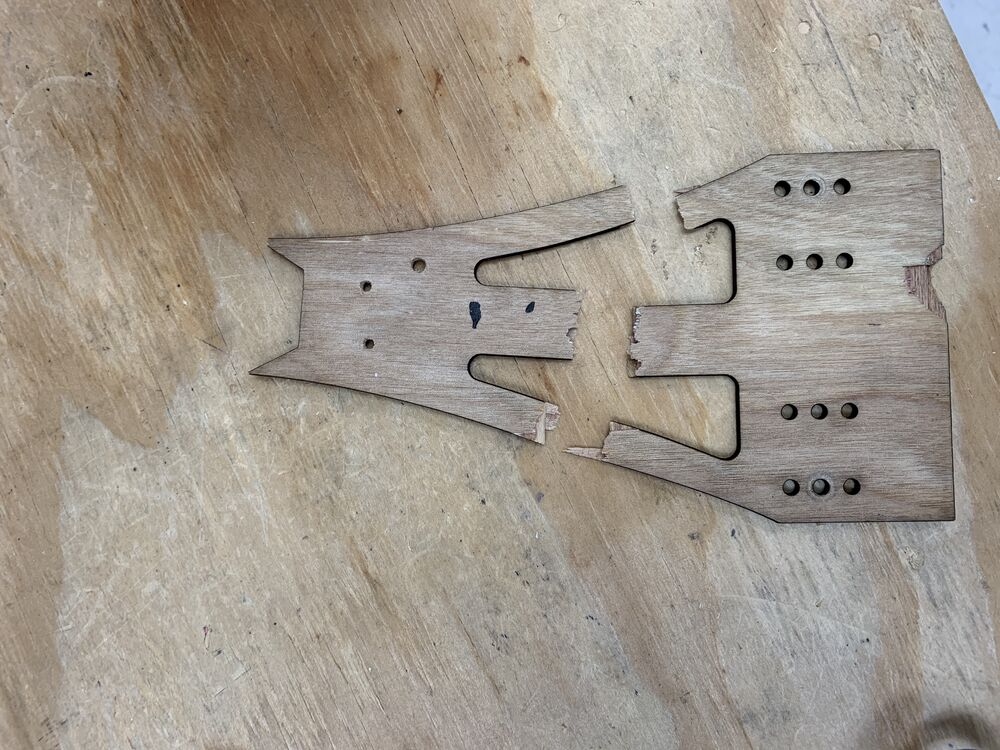
\includegraphics[width=0.95\textwidth]{Meetings/November/11-09-21/11-9-21_Hardware_Figure1 - Nathan Forrer.JPG}
  \caption{Our cracked backplate}
  \label{fig:pic1}
\end{minipage}%
\hfill%
\begin{minipage}[b]{.48\textwidth}
  \centering
  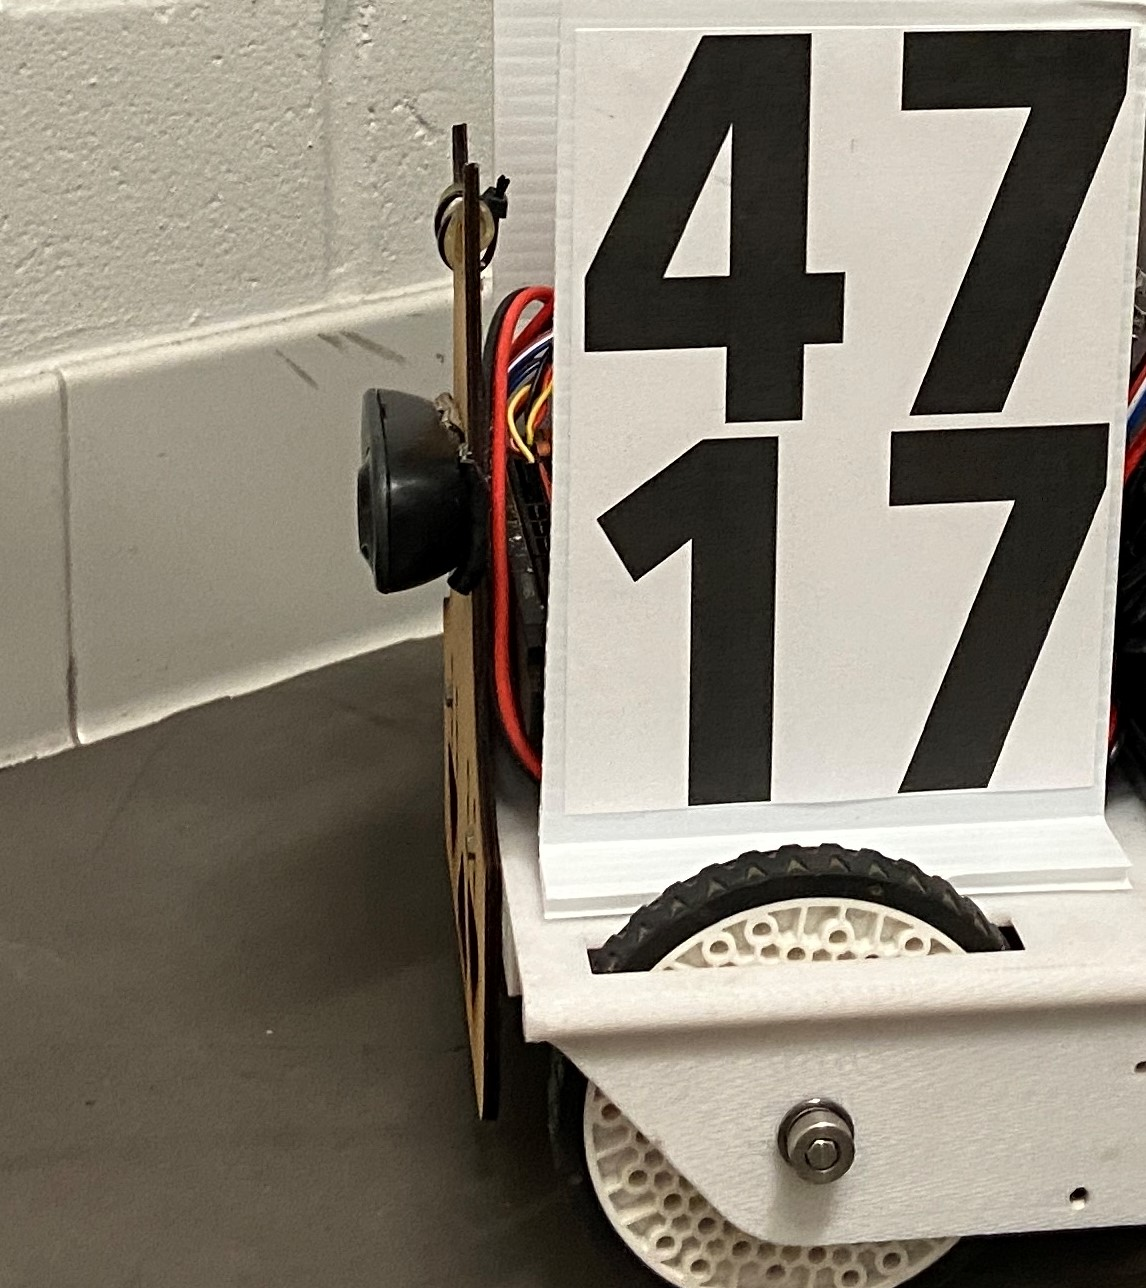
\includegraphics[width=0.95\textwidth]{Meetings/November/11-09-21/11-9-21_Hardware_Figure2 - Nathan Forrer.JPG}
  \caption{The camera isn't currently sitting flush with the robot}
  \label{fig:pic2}
\end{minipage}
\end{figure}

\begin{figure}[ht]
\centering
\begin{minipage}[b]{.48\textwidth}
  \centering
  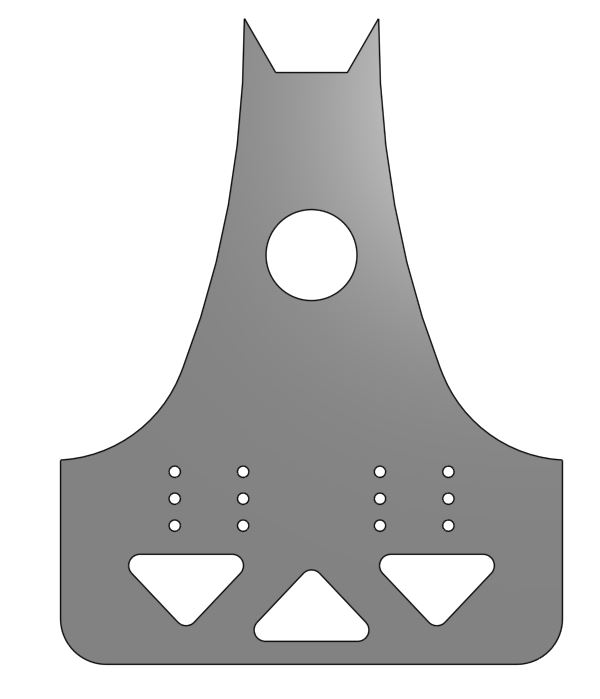
\includegraphics[width=0.95\textwidth]{Meetings/November/11-09-21/11-9-21_Hardware_Figure3 - Nathan Forrer.JPG}
  \caption{The new backplate}
  \label{fig:pic3}
\end{minipage}%
\hfill%
\begin{minipage}[b]{.48\textwidth}
  \centering
  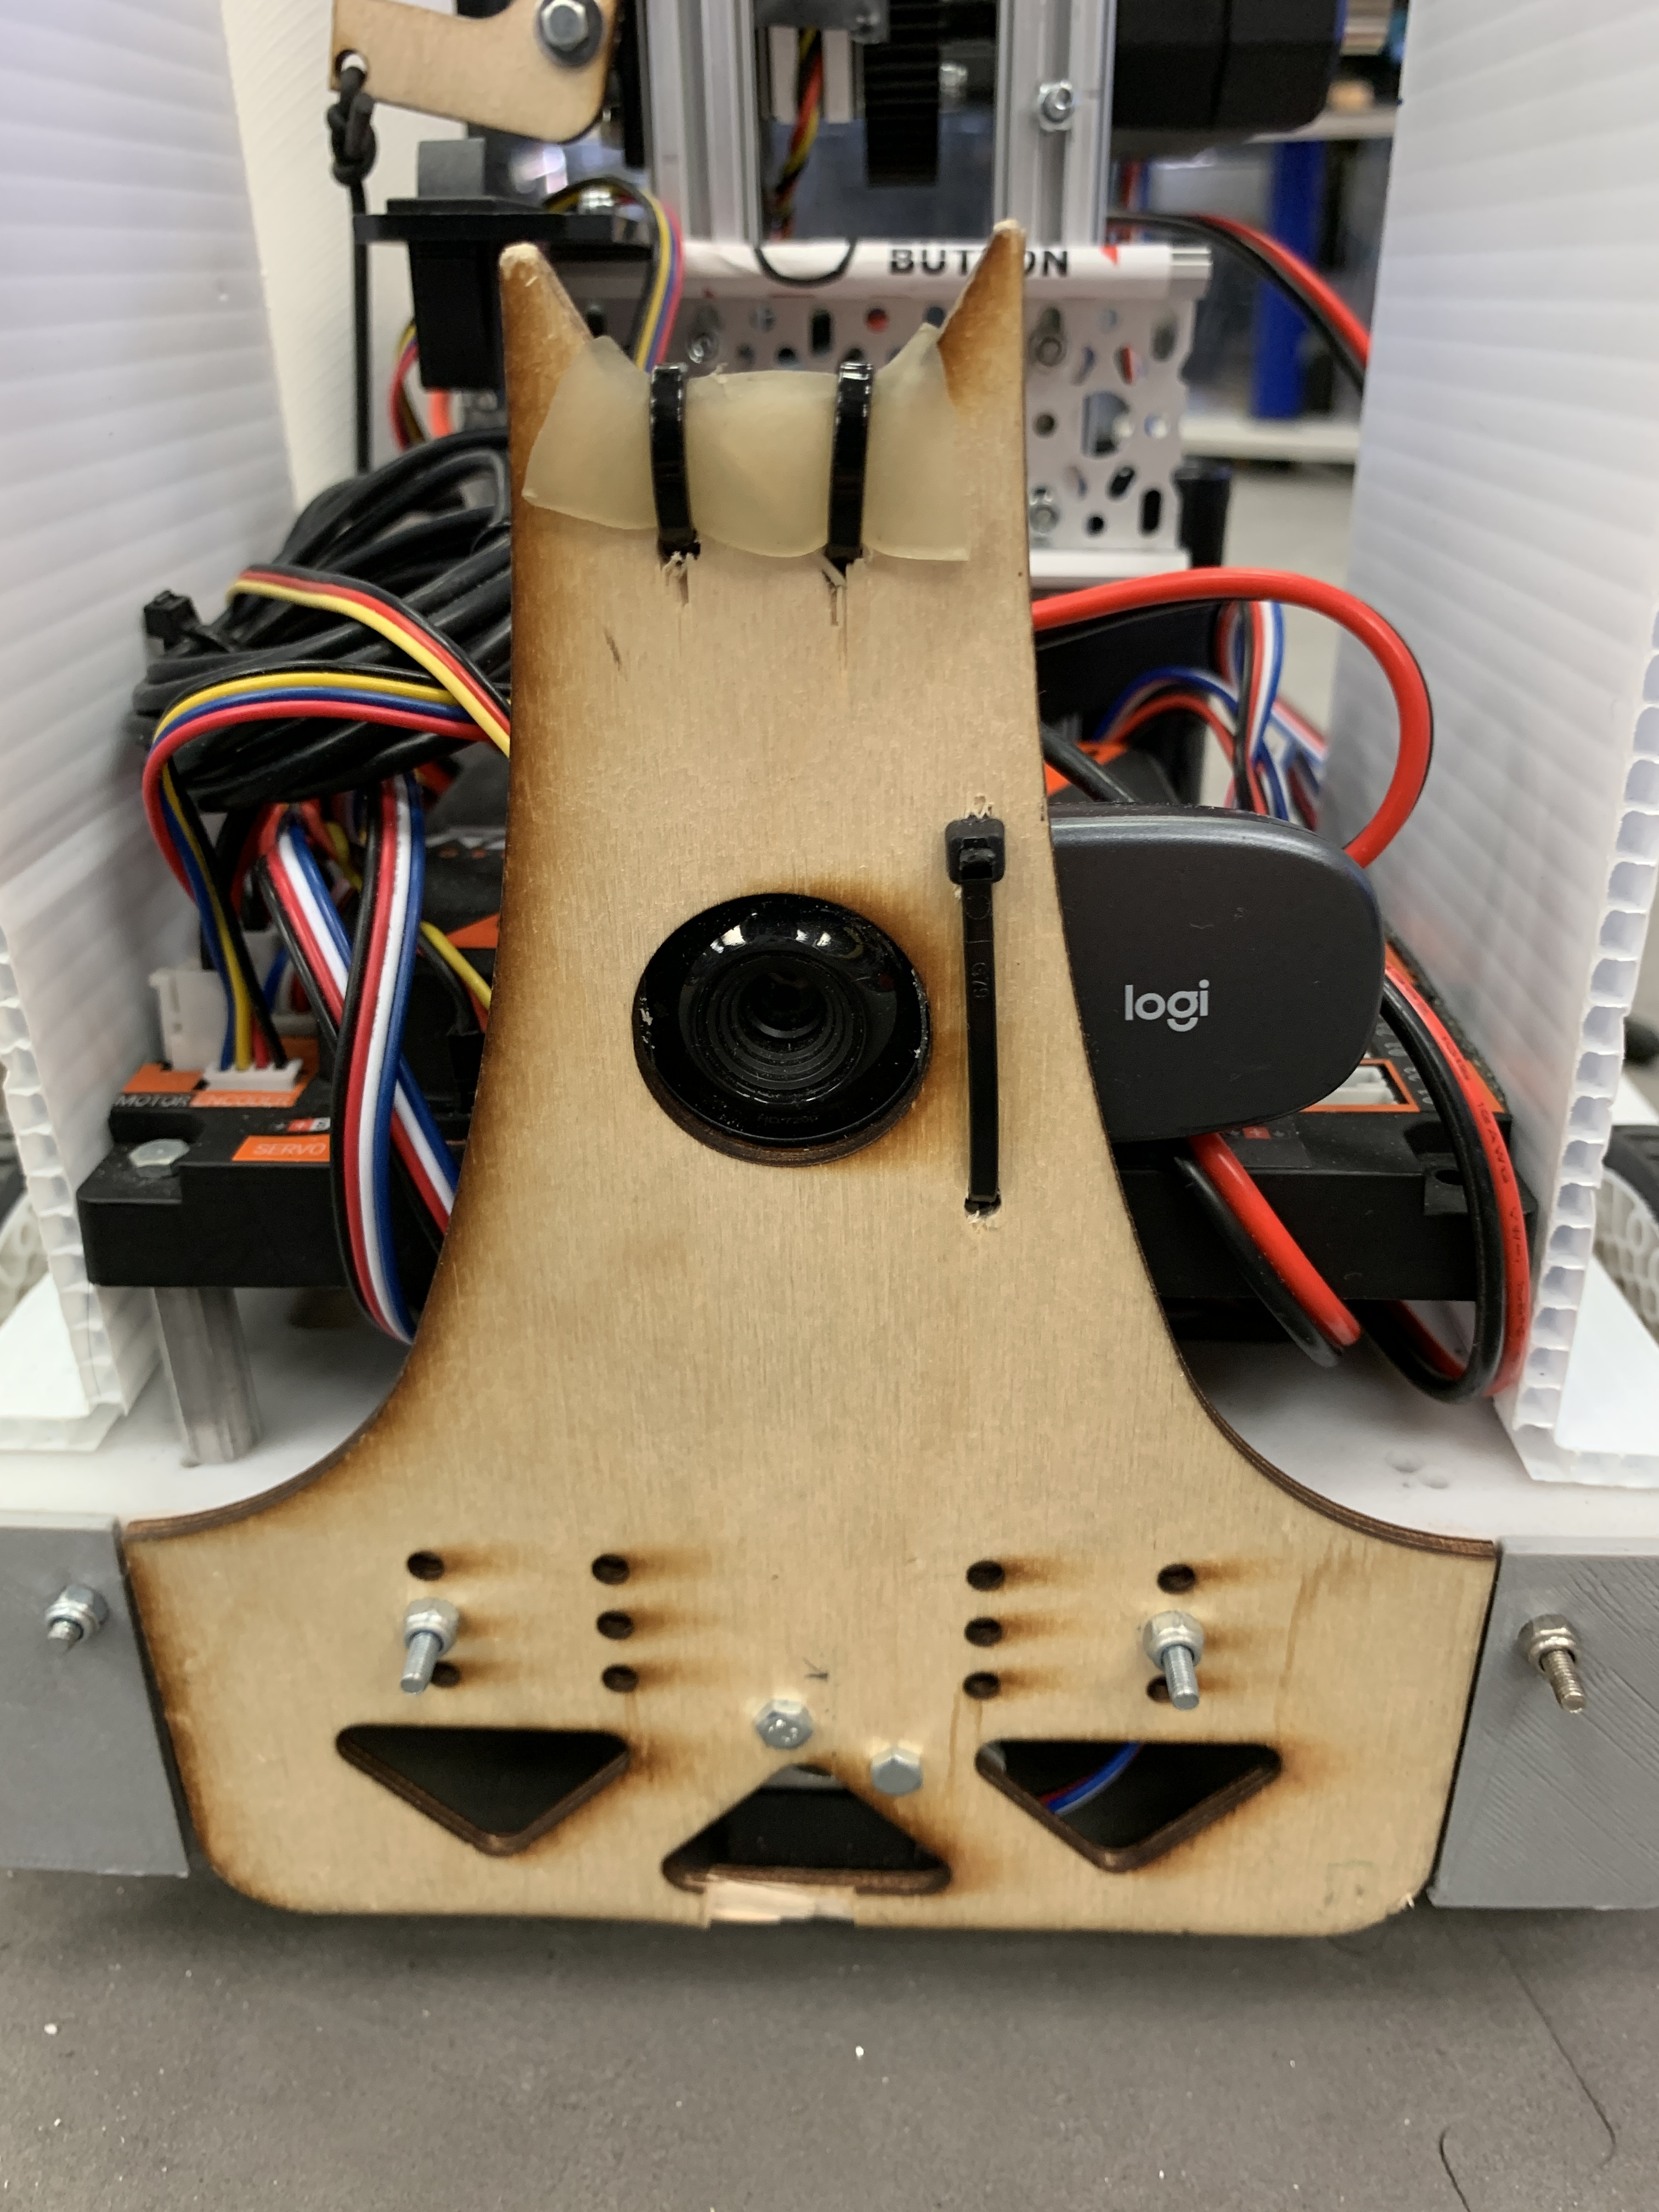
\includegraphics[width=0.95\textwidth]{Meetings/November/11-09-21/11-9-21_Hardware_Figure4 - Nathan Forrer.JPG}
  \caption{Cushioning impacts with surgical tubing}
  \label{fig:pic4}
\end{minipage}
\end{figure}

\whatsnext{
\begin{itemize}
    \item During the next meeting, our main priorities will be to design more buttons before our competition and to prepare our multimedia supplies for transportation to the location of the competition.
\end{itemize} 
}

